\documentclass[twoside]{book}

% Packages required by doxygen
\usepackage{fixltx2e}
\usepackage{calc}
\usepackage{doxygen}
\usepackage[export]{adjustbox} % also loads graphicx
\usepackage{graphicx}
\usepackage[utf8]{inputenc}
\usepackage{makeidx}
\usepackage{multicol}
\usepackage{multirow}
\PassOptionsToPackage{warn}{textcomp}
\usepackage{textcomp}
\usepackage[nointegrals]{wasysym}
\usepackage[table]{xcolor}

% Font selection
\usepackage[T1]{fontenc}
\usepackage[scaled=.90]{helvet}
\usepackage{courier}
\usepackage{amssymb}
\usepackage{sectsty}
\renewcommand{\familydefault}{\sfdefault}
\allsectionsfont{%
  \fontseries{bc}\selectfont%
  \color{darkgray}%
}
\renewcommand{\DoxyLabelFont}{%
  \fontseries{bc}\selectfont%
  \color{darkgray}%
}
\newcommand{\+}{\discretionary{\mbox{\scriptsize$\hookleftarrow$}}{}{}}

% Page & text layout
\usepackage{geometry}
\geometry{%
  a4paper,%
  top=2.5cm,%
  bottom=2.5cm,%
  left=2.5cm,%
  right=2.5cm%
}
\tolerance=750
\hfuzz=15pt
\hbadness=750
\setlength{\emergencystretch}{15pt}
\setlength{\parindent}{0cm}
\setlength{\parskip}{0.2cm}
\makeatletter
\renewcommand{\paragraph}{%
  \@startsection{paragraph}{4}{0ex}{-1.0ex}{1.0ex}{%
    \normalfont\normalsize\bfseries\SS@parafont%
  }%
}
\renewcommand{\subparagraph}{%
  \@startsection{subparagraph}{5}{0ex}{-1.0ex}{1.0ex}{%
    \normalfont\normalsize\bfseries\SS@subparafont%
  }%
}
\makeatother

% Headers & footers
\usepackage{fancyhdr}
\pagestyle{fancyplain}
\fancyhead[LE]{\fancyplain{}{\bfseries\thepage}}
\fancyhead[CE]{\fancyplain{}{}}
\fancyhead[RE]{\fancyplain{}{\bfseries\leftmark}}
\fancyhead[LO]{\fancyplain{}{\bfseries\rightmark}}
\fancyhead[CO]{\fancyplain{}{}}
\fancyhead[RO]{\fancyplain{}{\bfseries\thepage}}
\fancyfoot[LE]{\fancyplain{}{}}
\fancyfoot[CE]{\fancyplain{}{}}
\fancyfoot[RE]{\fancyplain{}{\bfseries\scriptsize Generated on Fri Apr 8 2016 15\+:00\+:40 for map by Doxygen }}
\fancyfoot[LO]{\fancyplain{}{\bfseries\scriptsize Generated on Fri Apr 8 2016 15\+:00\+:40 for map by Doxygen }}
\fancyfoot[CO]{\fancyplain{}{}}
\fancyfoot[RO]{\fancyplain{}{}}
\renewcommand{\footrulewidth}{0.4pt}
\renewcommand{\chaptermark}[1]{%
  \markboth{#1}{}%
}
\renewcommand{\sectionmark}[1]{%
  \markright{\thesection\ #1}%
}

% Indices & bibliography
\usepackage{natbib}
\usepackage[titles]{tocloft}
\setcounter{tocdepth}{3}
\setcounter{secnumdepth}{5}
\makeindex

% Hyperlinks (required, but should be loaded last)
\usepackage{ifpdf}
\ifpdf
  \usepackage[pdftex,pagebackref=true]{hyperref}
\else
  \usepackage[ps2pdf,pagebackref=true]{hyperref}
\fi
\hypersetup{%
  colorlinks=true,%
  linkcolor=blue,%
  citecolor=blue,%
  unicode%
}

% Custom commands
\newcommand{\clearemptydoublepage}{%
  \newpage{\pagestyle{empty}\cleardoublepage}%
}


%===== C O N T E N T S =====

\begin{document}

% Titlepage & ToC
\hypersetup{pageanchor=false,
             bookmarks=true,
             bookmarksnumbered=true,
             pdfencoding=unicode
            }
\pagenumbering{roman}
\begin{titlepage}
\vspace*{7cm}
\begin{center}%
{\Large map }\\
\vspace*{1cm}
{\large Generated by Doxygen 1.8.10}\\
\vspace*{0.5cm}
{\small Fri Apr 8 2016 15:00:40}\\
\end{center}
\end{titlepage}
\clearemptydoublepage
\tableofcontents
\clearemptydoublepage
\pagenumbering{arabic}
\hypersetup{pageanchor=true}

%--- Begin generated contents ---
\chapter{Namespace Index}
\section{Namespace List}
Here is a list of all documented namespaces with brief descriptions\+:\begin{DoxyCompactList}
\item\contentsline{section}{\hyperlink{namespacer2d2}{r2d2} \\*Map\+Interface is a interface for maps to retrieve and save information about a certain area. The interface makes sure, no matter what type of map is created, the info about that map is given in the same format }{\pageref{namespacer2d2}}{}
\end{DoxyCompactList}

\chapter{Hierarchical Index}
\section{Class Hierarchy}
This inheritance list is sorted roughly, but not completely, alphabetically\+:\begin{DoxyCompactList}
\item \contentsline{section}{r2d2\+:\+:Box\+Info}{\pageref{classr2d2_1_1_box_info}}{}
\item \contentsline{section}{r2d2\+:\+:Read\+Only\+Map}{\pageref{classr2d2_1_1_read_only_map}}{}
\begin{DoxyCompactList}
\item \contentsline{section}{r2d2\+:\+:Read\+Write\+Map}{\pageref{classr2d2_1_1_read_write_map}}{}
\begin{DoxyCompactList}
\item \contentsline{section}{r2d2\+:\+:Save\+Load\+Map}{\pageref{classr2d2_1_1_save_load_map}}{}
\begin{DoxyCompactList}
\item \contentsline{section}{r2d2\+:\+:Box\+Map}{\pageref{classr2d2_1_1_box_map}}{}
\end{DoxyCompactList}
\end{DoxyCompactList}
\end{DoxyCompactList}
\end{DoxyCompactList}

\chapter{Class Index}
\section{Class List}
Here are the classes, structs, unions and interfaces with brief descriptions\+:\begin{DoxyCompactList}
\item\contentsline{section}{\hyperlink{classr2d2_1_1_box_info}{r2d2\+::\+Box\+Info} }{\pageref{classr2d2_1_1_box_info}}{}
\item\contentsline{section}{\hyperlink{classr2d2_1_1_box_map}{r2d2\+::\+Box\+Map} }{\pageref{classr2d2_1_1_box_map}}{}
\item\contentsline{section}{\hyperlink{classr2d2_1_1_read_only_map}{r2d2\+::\+Read\+Only\+Map} }{\pageref{classr2d2_1_1_read_only_map}}{}
\item\contentsline{section}{\hyperlink{classr2d2_1_1_read_write_map}{r2d2\+::\+Read\+Write\+Map} }{\pageref{classr2d2_1_1_read_write_map}}{}
\item\contentsline{section}{\hyperlink{classr2d2_1_1_save_load_map}{r2d2\+::\+Save\+Load\+Map} }{\pageref{classr2d2_1_1_save_load_map}}{}
\end{DoxyCompactList}

\chapter{Namespace Documentation}
\hypertarget{namespacer2d2}{}\section{r2d2 Namespace Reference}
\label{namespacer2d2}\index{r2d2@{r2d2}}


Map\+Interface is a interface for maps to retrieve and save information about a certain area. The interface makes sure, no matter what type of map is created, the info about that map is given in the same format.  


\subsection*{Classes}
\begin{DoxyCompactItemize}
\item 
class \hyperlink{classr2d2_1_1_box_info}{Box\+Info}
\item 
class \hyperlink{classr2d2_1_1_box_map}{Box\+Map}
\item 
class \hyperlink{classr2d2_1_1_read_only_map}{Read\+Only\+Map}
\item 
class \hyperlink{classr2d2_1_1_read_write_map}{Read\+Write\+Map}
\item 
class \hyperlink{classr2d2_1_1_save_load_map}{Save\+Load\+Map}
\end{DoxyCompactItemize}


\subsection{Detailed Description}
Map\+Interface is a interface for maps to retrieve and save information about a certain area. The interface makes sure, no matter what type of map is created, the info about that map is given in the same format. 

\begin{DoxyAuthor}{Author}
Sander Kolman 
\end{DoxyAuthor}
\begin{DoxyDate}{Date}
08-\/04-\/16 
\end{DoxyDate}
\begin{DoxyVersion}{Version}
1.\+0 The interface is split up in 3 different classes. These classes are meant for more structured and safe usage.
\begin{DoxyItemize}
\item \hyperlink{classr2d2_1_1_read_only_map}{Read\+Only\+Map} is the simplest interface, only allowing read functionality.
\item \hyperlink{classr2d2_1_1_read_write_map}{Read\+Write\+Map} inherits the functionality of the above, it also adds a write function to fill a map with data.
\item \hyperlink{classr2d2_1_1_save_load_map}{Save\+Load\+Map} inherits the functionality of the above, it also adds functions to save and load a map respectivly to and from file I/\+O.
\end{DoxyItemize}
\end{DoxyVersion}
The fourth class defined is the data that will actually be captured about a certain area. It contains 3 boolean attributes for different information about an area.

For example\+: 
\begin{DoxyCodeInclude}
\textcolor{keywordtype}{void} make\_map\_interface()\{
    \hyperlink{classr2d2_1_1_read_write_map}{r2d2::ReadWriteMap} * map = \textcolor{keyword}{new} \hyperlink{classr2d2_1_1_box_map}{r2d2::BoxMap}\{\};
    map->\hyperlink{classr2d2_1_1_read_write_map_a8169c7a36a66b824403a4df7a91d232d}{set\_box\_info}(random\_box(), \hyperlink{classr2d2_1_1_box_info}{r2d2::BoxInfo}\{\});
    cout << map->\hyperlink{classr2d2_1_1_read_only_map_a322efcf80b3f461769e69cbb60a87b72}{get\_map\_bounding\_box}() << endl;
    \textcolor{keyword}{delete} map;
\}
\end{DoxyCodeInclude}

\chapter{Class Documentation}
\hypertarget{classr2d2_1_1_box_info}{}\section{r2d2\+:\+:Box\+Info Class Reference}
\label{classr2d2_1_1_box_info}\index{r2d2\+::\+Box\+Info@{r2d2\+::\+Box\+Info}}
\subsection*{Public Member Functions}
\begin{DoxyCompactItemize}
\item 
\hyperlink{classr2d2_1_1_box_info_aecb228ad1f7d71ef89b22eaf9fb91353}{Box\+Info} (bool has\+\_\+obstacle=false, bool has\+\_\+unknown=false, bool has\+\_\+navigatable=false)
\begin{DoxyCompactList}\small\item\em Constructor for \hyperlink{classr2d2_1_1_box_info}{Box\+Info}. \end{DoxyCompactList}\item 
bool \hyperlink{classr2d2_1_1_box_info_a1acf6db4b90ea6a7cb405ab2dfe1237e}{get\+\_\+has\+\_\+obstacle} () const 
\begin{DoxyCompactList}\small\item\em Getter for obstacle bool. \end{DoxyCompactList}\item 
bool \hyperlink{classr2d2_1_1_box_info_a3a7e5f644442d123f2e07651442bc8d6}{get\+\_\+has\+\_\+unknown} () const 
\begin{DoxyCompactList}\small\item\em Getter for unknown bool. \end{DoxyCompactList}\item 
bool \hyperlink{classr2d2_1_1_box_info_ac7793568145b5e3931e2061bb4fb2f1a}{get\+\_\+has\+\_\+navigatable} () const 
\begin{DoxyCompactList}\small\item\em Getter for navigatable bool. \end{DoxyCompactList}\item 
bool \hyperlink{classr2d2_1_1_box_info_acfea2fcf06c42d765fe7fc6048101782}{operator==} (const \hyperlink{classr2d2_1_1_box_info}{Box\+Info} rhs) const 
\item 
bool \hyperlink{classr2d2_1_1_box_info_aa6021b526eb5e161f56bc6cfbf031f89}{operator!=} (const \hyperlink{classr2d2_1_1_box_info}{Box\+Info} rhs) const 
\end{DoxyCompactItemize}


\subsection{Constructor \& Destructor Documentation}
\hypertarget{classr2d2_1_1_box_info_aecb228ad1f7d71ef89b22eaf9fb91353}{}\index{r2d2\+::\+Box\+Info@{r2d2\+::\+Box\+Info}!Box\+Info@{Box\+Info}}
\index{Box\+Info@{Box\+Info}!r2d2\+::\+Box\+Info@{r2d2\+::\+Box\+Info}}
\subsubsection[{Box\+Info(bool has\+\_\+obstacle=false, bool has\+\_\+unknown=false, bool has\+\_\+navigatable=false)}]{\setlength{\rightskip}{0pt plus 5cm}r2d2\+::\+Box\+Info\+::\+Box\+Info (
\begin{DoxyParamCaption}
\item[{bool}]{has\+\_\+obstacle = {\ttfamily false}, }
\item[{bool}]{has\+\_\+unknown = {\ttfamily false}, }
\item[{bool}]{has\+\_\+navigatable = {\ttfamily false}}
\end{DoxyParamCaption}
)}\label{classr2d2_1_1_box_info_aecb228ad1f7d71ef89b22eaf9fb91353}


Constructor for \hyperlink{classr2d2_1_1_box_info}{Box\+Info}. 


\begin{DoxyParams}{Parameters}
{\em has\+\_\+obstacle} & bool describing if box has an obstacle, default\+: false. \\
\hline
{\em has\+\_\+unknown} & bool describing if box has an obstacle, default\+: false. \\
\hline
{\em has\+\_\+navigatable} & bool describing if box has an obstacle, default\+: false. \\
\hline
\end{DoxyParams}


\subsection{Member Function Documentation}
\hypertarget{classr2d2_1_1_box_info_ac7793568145b5e3931e2061bb4fb2f1a}{}\index{r2d2\+::\+Box\+Info@{r2d2\+::\+Box\+Info}!get\+\_\+has\+\_\+navigatable@{get\+\_\+has\+\_\+navigatable}}
\index{get\+\_\+has\+\_\+navigatable@{get\+\_\+has\+\_\+navigatable}!r2d2\+::\+Box\+Info@{r2d2\+::\+Box\+Info}}
\subsubsection[{get\+\_\+has\+\_\+navigatable() const }]{\setlength{\rightskip}{0pt plus 5cm}bool r2d2\+::\+Box\+Info\+::get\+\_\+has\+\_\+navigatable (
\begin{DoxyParamCaption}
{}
\end{DoxyParamCaption}
) const}\label{classr2d2_1_1_box_info_ac7793568145b5e3931e2061bb4fb2f1a}


Getter for navigatable bool. 

\begin{DoxyReturn}{Returns}
const bool Box\+Info\+::has\+\_\+navigatable 
\end{DoxyReturn}
\hypertarget{classr2d2_1_1_box_info_a1acf6db4b90ea6a7cb405ab2dfe1237e}{}\index{r2d2\+::\+Box\+Info@{r2d2\+::\+Box\+Info}!get\+\_\+has\+\_\+obstacle@{get\+\_\+has\+\_\+obstacle}}
\index{get\+\_\+has\+\_\+obstacle@{get\+\_\+has\+\_\+obstacle}!r2d2\+::\+Box\+Info@{r2d2\+::\+Box\+Info}}
\subsubsection[{get\+\_\+has\+\_\+obstacle() const }]{\setlength{\rightskip}{0pt plus 5cm}bool r2d2\+::\+Box\+Info\+::get\+\_\+has\+\_\+obstacle (
\begin{DoxyParamCaption}
{}
\end{DoxyParamCaption}
) const}\label{classr2d2_1_1_box_info_a1acf6db4b90ea6a7cb405ab2dfe1237e}


Getter for obstacle bool. 

\begin{DoxyReturn}{Returns}
const bool Box\+Info\+::has\+\_\+obstacle 
\end{DoxyReturn}
\hypertarget{classr2d2_1_1_box_info_a3a7e5f644442d123f2e07651442bc8d6}{}\index{r2d2\+::\+Box\+Info@{r2d2\+::\+Box\+Info}!get\+\_\+has\+\_\+unknown@{get\+\_\+has\+\_\+unknown}}
\index{get\+\_\+has\+\_\+unknown@{get\+\_\+has\+\_\+unknown}!r2d2\+::\+Box\+Info@{r2d2\+::\+Box\+Info}}
\subsubsection[{get\+\_\+has\+\_\+unknown() const }]{\setlength{\rightskip}{0pt plus 5cm}bool r2d2\+::\+Box\+Info\+::get\+\_\+has\+\_\+unknown (
\begin{DoxyParamCaption}
{}
\end{DoxyParamCaption}
) const}\label{classr2d2_1_1_box_info_a3a7e5f644442d123f2e07651442bc8d6}


Getter for unknown bool. 

\begin{DoxyReturn}{Returns}
const bool Box\+Info\+::has\+\_\+unknown 
\end{DoxyReturn}
\hypertarget{classr2d2_1_1_box_info_aa6021b526eb5e161f56bc6cfbf031f89}{}\index{r2d2\+::\+Box\+Info@{r2d2\+::\+Box\+Info}!operator"!=@{operator"!=}}
\index{operator"!=@{operator"!=}!r2d2\+::\+Box\+Info@{r2d2\+::\+Box\+Info}}
\subsubsection[{operator"!=(const Box\+Info rhs) const }]{\setlength{\rightskip}{0pt plus 5cm}bool r2d2\+::\+Box\+Info\+::operator!= (
\begin{DoxyParamCaption}
\item[{const {\bf Box\+Info}}]{rhs}
\end{DoxyParamCaption}
) const}\label{classr2d2_1_1_box_info_aa6021b526eb5e161f56bc6cfbf031f89}
The operator != (not equal)

Exact inverse of \hyperlink{classr2d2_1_1_box_info_acfea2fcf06c42d765fe7fc6048101782}{operator==()}. 
\begin{DoxyParams}{Parameters}
{\em rhs} & const \hyperlink{classr2d2_1_1_box_info}{Box\+Info} object. \\
\hline
\end{DoxyParams}
\begin{DoxyReturn}{Returns}
bool, true if \hyperlink{classr2d2_1_1_box_info_acfea2fcf06c42d765fe7fc6048101782}{operator==()} is false. 
\end{DoxyReturn}
\hypertarget{classr2d2_1_1_box_info_acfea2fcf06c42d765fe7fc6048101782}{}\index{r2d2\+::\+Box\+Info@{r2d2\+::\+Box\+Info}!operator==@{operator==}}
\index{operator==@{operator==}!r2d2\+::\+Box\+Info@{r2d2\+::\+Box\+Info}}
\subsubsection[{operator==(const Box\+Info rhs) const }]{\setlength{\rightskip}{0pt plus 5cm}bool r2d2\+::\+Box\+Info\+::operator== (
\begin{DoxyParamCaption}
\item[{const {\bf Box\+Info}}]{rhs}
\end{DoxyParamCaption}
) const}\label{classr2d2_1_1_box_info_acfea2fcf06c42d765fe7fc6048101782}
The operator == (is equal)

Check if 2 \hyperlink{classr2d2_1_1_box_info}{Box\+Info}\textquotesingle{}s are completely equal. 
\begin{DoxyParams}{Parameters}
{\em rhs} & const \hyperlink{classr2d2_1_1_box_info}{Box\+Info} object. \\
\hline
\end{DoxyParams}
\begin{DoxyReturn}{Returns}
bool, true if all internal bools are equal. 
\end{DoxyReturn}


The documentation for this class was generated from the following files\+:\begin{DoxyCompactItemize}
\item 
source/include/Map\+Interface.\+hpp\item 
source/src/Map\+Interface.\+cpp\end{DoxyCompactItemize}

\hypertarget{classr2d2_1_1_box_map}{}\section{r2d2\+:\+:Box\+Map Class Reference}
\label{classr2d2_1_1_box_map}\index{r2d2\+::\+Box\+Map@{r2d2\+::\+Box\+Map}}
Inheritance diagram for r2d2\+:\+:Box\+Map\+:\begin{figure}[H]
\begin{center}
\leavevmode
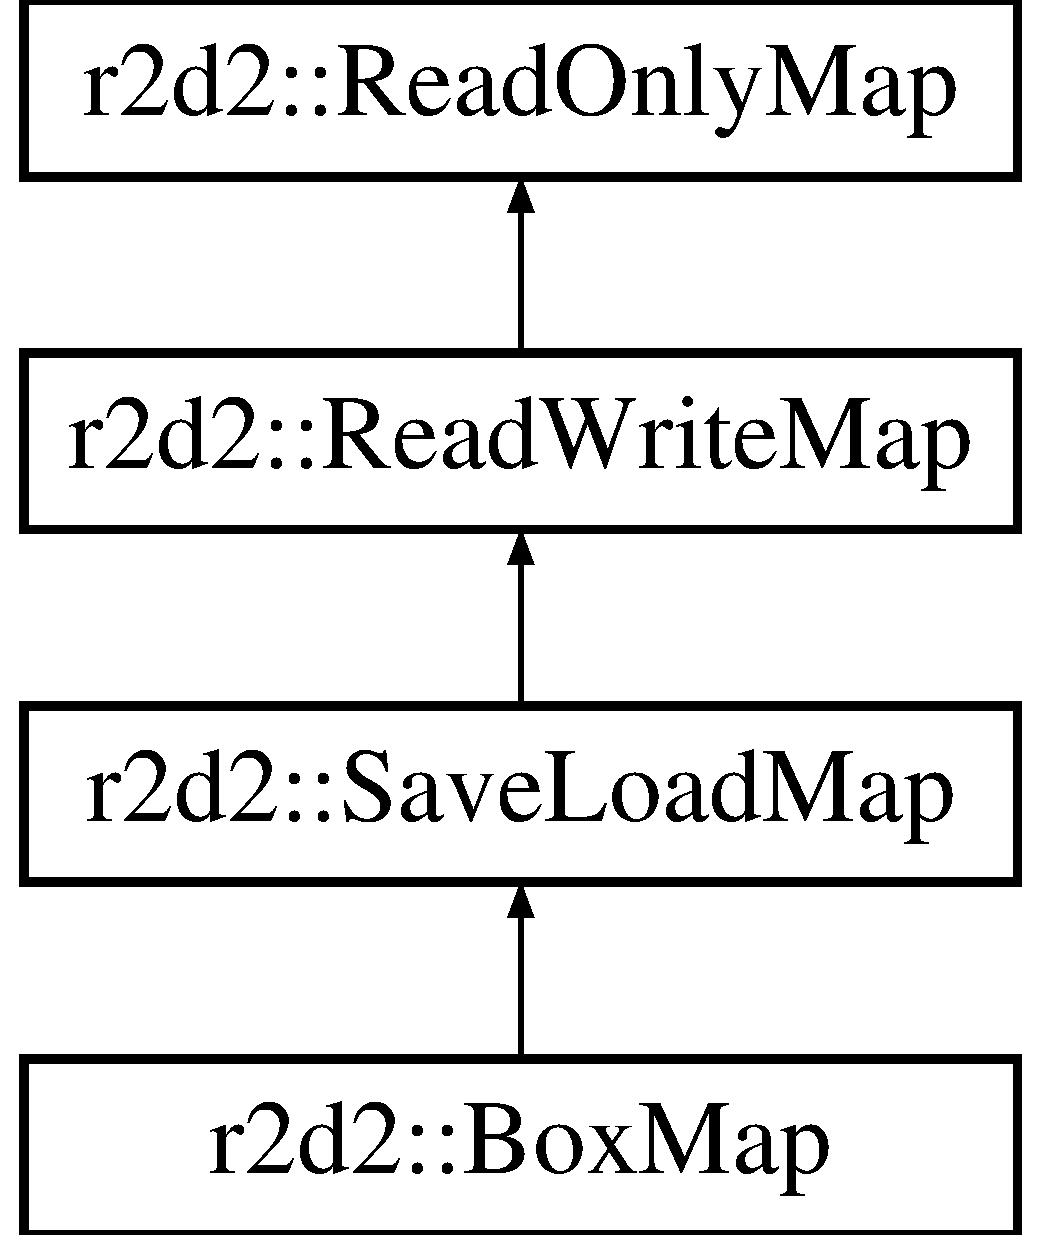
\includegraphics[height=4.000000cm]{classr2d2_1_1_box_map}
\end{center}
\end{figure}
\subsection*{Public Member Functions}
\begin{DoxyCompactItemize}
\item 
const \hyperlink{classr2d2_1_1_box_info}{Box\+Info} \hyperlink{classr2d2_1_1_box_map_aa6fd512737ad45da9bc46a516807f71e}{get\+\_\+box\+\_\+info} (const Box box) override
\begin{DoxyCompactList}\small\item\em Get Box information about a certain area. All bools are false if no information is found, overwritten with true if true is found in the map. \end{DoxyCompactList}\item 
const Box \hyperlink{classr2d2_1_1_box_map_ac1aea64a58cdb6916ecbcb0d2ea780c2}{get\+\_\+map\+\_\+bounding\+\_\+box} () override
\begin{DoxyCompactList}\small\item\em Scans all boxes in the map and makes a box precisely around all other boxes. \end{DoxyCompactList}\item 
void \hyperlink{classr2d2_1_1_box_map_ac421b31be9f2e2248127f21f3299883d}{set\+\_\+box\+\_\+info} (const Box box, const \hyperlink{classr2d2_1_1_box_info}{Box\+Info} box\+\_\+info) override
\begin{DoxyCompactList}\small\item\em Places a new box in the map with \hyperlink{classr2d2_1_1_box_info}{Box\+Info}. \end{DoxyCompactList}\item 
void \hyperlink{classr2d2_1_1_box_map_a23970768a8508c94ba88be91ab87d4ac}{save} (std\+::string filename) override
\begin{DoxyCompactList}\small\item\em Saves the data of a \hyperlink{classr2d2_1_1_box_map}{Box\+Map} to a json file. \end{DoxyCompactList}\item 
void \hyperlink{classr2d2_1_1_box_map_a4bc5818e4802d2d1b0a66c0d6c2bb0d0}{load} (std\+::string filename) override
\begin{DoxyCompactList}\small\item\em Loads the data of a json file to a \hyperlink{classr2d2_1_1_box_map}{Box\+Map}. \end{DoxyCompactList}\item 
\hypertarget{classr2d2_1_1_box_map_a2d5e901a18b8402156a9c29d802b0b06}{}int {\bfseries get\+\_\+map\+\_\+size} ()\label{classr2d2_1_1_box_map_a2d5e901a18b8402156a9c29d802b0b06}

\end{DoxyCompactItemize}


\subsection{Member Function Documentation}
\hypertarget{classr2d2_1_1_box_map_aa6fd512737ad45da9bc46a516807f71e}{}\index{r2d2\+::\+Box\+Map@{r2d2\+::\+Box\+Map}!get\+\_\+box\+\_\+info@{get\+\_\+box\+\_\+info}}
\index{get\+\_\+box\+\_\+info@{get\+\_\+box\+\_\+info}!r2d2\+::\+Box\+Map@{r2d2\+::\+Box\+Map}}
\subsubsection[{get\+\_\+box\+\_\+info(const Box box) override}]{\setlength{\rightskip}{0pt plus 5cm}const {\bf Box\+Info} r2d2\+::\+Box\+Map\+::get\+\_\+box\+\_\+info (
\begin{DoxyParamCaption}
\item[{const Box}]{box}
\end{DoxyParamCaption}
)\hspace{0.3cm}{\ttfamily [override]}, {\ttfamily [virtual]}}\label{classr2d2_1_1_box_map_aa6fd512737ad45da9bc46a516807f71e}


Get Box information about a certain area. All bools are false if no information is found, overwritten with true if true is found in the map. 

Get Box Information.


\begin{DoxyParams}{Parameters}
{\em box} & The area that is to be checked. \\
\hline
\end{DoxyParams}
\begin{DoxyReturn}{Returns}
\hyperlink{classr2d2_1_1_box_info}{Box\+Info}, the found information about the area. 
\end{DoxyReturn}


Implements \hyperlink{classr2d2_1_1_read_only_map_ae088c8f8cea0870bf3db8bbf3a0821b8}{r2d2\+::\+Read\+Only\+Map}.

\hypertarget{classr2d2_1_1_box_map_ac1aea64a58cdb6916ecbcb0d2ea780c2}{}\index{r2d2\+::\+Box\+Map@{r2d2\+::\+Box\+Map}!get\+\_\+map\+\_\+bounding\+\_\+box@{get\+\_\+map\+\_\+bounding\+\_\+box}}
\index{get\+\_\+map\+\_\+bounding\+\_\+box@{get\+\_\+map\+\_\+bounding\+\_\+box}!r2d2\+::\+Box\+Map@{r2d2\+::\+Box\+Map}}
\subsubsection[{get\+\_\+map\+\_\+bounding\+\_\+box() override}]{\setlength{\rightskip}{0pt plus 5cm}const Box r2d2\+::\+Box\+Map\+::get\+\_\+map\+\_\+bounding\+\_\+box (
\begin{DoxyParamCaption}
{}
\end{DoxyParamCaption}
)\hspace{0.3cm}{\ttfamily [override]}, {\ttfamily [virtual]}}\label{classr2d2_1_1_box_map_ac1aea64a58cdb6916ecbcb0d2ea780c2}


Scans all boxes in the map and makes a box precisely around all other boxes. 

Get the Box containing all boxes in the current map.

\begin{DoxyReturn}{Returns}
const Box, the box containing all other boxes. 
\end{DoxyReturn}


Implements \hyperlink{classr2d2_1_1_read_only_map_a322efcf80b3f461769e69cbb60a87b72}{r2d2\+::\+Read\+Only\+Map}.

\hypertarget{classr2d2_1_1_box_map_a4bc5818e4802d2d1b0a66c0d6c2bb0d0}{}\index{r2d2\+::\+Box\+Map@{r2d2\+::\+Box\+Map}!load@{load}}
\index{load@{load}!r2d2\+::\+Box\+Map@{r2d2\+::\+Box\+Map}}
\subsubsection[{load(std\+::string filename) override}]{\setlength{\rightskip}{0pt plus 5cm}void r2d2\+::\+Box\+Map\+::load (
\begin{DoxyParamCaption}
\item[{std\+::string}]{filename}
\end{DoxyParamCaption}
)\hspace{0.3cm}{\ttfamily [override]}, {\ttfamily [virtual]}}\label{classr2d2_1_1_box_map_a4bc5818e4802d2d1b0a66c0d6c2bb0d0}


Loads the data of a json file to a \hyperlink{classr2d2_1_1_box_map}{Box\+Map}. 


\begin{DoxyParams}{Parameters}
{\em filename} & the destination of the file that needs to be loaded \\
\hline
\end{DoxyParams}
Open file

Push contents into D\+O\+M element

Allocate element\+\_\+size

Load values from D\+O\+M element

Close file 

Implements \hyperlink{classr2d2_1_1_save_load_map}{r2d2\+::\+Save\+Load\+Map}.

\hypertarget{classr2d2_1_1_box_map_a23970768a8508c94ba88be91ab87d4ac}{}\index{r2d2\+::\+Box\+Map@{r2d2\+::\+Box\+Map}!save@{save}}
\index{save@{save}!r2d2\+::\+Box\+Map@{r2d2\+::\+Box\+Map}}
\subsubsection[{save(std\+::string filename) override}]{\setlength{\rightskip}{0pt plus 5cm}void r2d2\+::\+Box\+Map\+::save (
\begin{DoxyParamCaption}
\item[{std\+::string}]{filename}
\end{DoxyParamCaption}
)\hspace{0.3cm}{\ttfamily [override]}, {\ttfamily [virtual]}}\label{classr2d2_1_1_box_map_a23970768a8508c94ba88be91ab87d4ac}


Saves the data of a \hyperlink{classr2d2_1_1_box_map}{Box\+Map} to a json file. 


\begin{DoxyParams}{Parameters}
{\em filename} & the destination of the file \\
\hline
\end{DoxyParams}
Create a D\+O\+M document

Create the first level of json \{ \char`\"{}left\+\_\+coordinates\char`\"{}\+:\mbox{[}\{\}\mbox{]}, \char`\"{}right\+\_\+coordinates\char`\"{}\+:\mbox{[}\{\}\mbox{]}, \char`\"{}box\+\_\+infos\char`\"{}\+:\mbox{[}\{\}\mbox{]} \}

Create coordinate placeholders \char`\"{}left\+\_\+coordinates\char`\"{}\+:\mbox{[}\{\char`\"{}x\char`\"{}\+:left\+\_\+coordinate\+\_\+x,\char`\"{}y\char`\"{}\+:left\+\_\+coordinate\+\_\+y,\char`\"{}z\char`\"{}\+:left\+\_\+coordinate\+\_\+z\}\mbox{]}

Create coordinate placeholders \char`\"{}right\+\_\+coordinates\char`\"{}\+:\mbox{[}\{\char`\"{}x\char`\"{}\+:right\+\_\+coordinate\+\_\+x,\char`\"{}y\char`\"{}\+:right\+\_\+coordinate\+\_\+y,\char`\"{}z\char`\"{}\+:right\+\_\+coordinate\+\_\+z\}\mbox{]}

Create box\+\_\+info placeholders \char`\"{}box\+\_\+infos\char`\"{}\+:\mbox{[}\{\char`\"{}has\+\_\+obstacle\char`\"{}\+:has\+\_\+obstacle,\char`\"{}has\+\_\+unknown\char`\"{}\+:has\+\_\+unknown,\char`\"{}has\+\_\+navigatable\char`\"{}\+:has\+\_\+navigatable\}\mbox{]}

Add indexes to Objects

Push object to their destination array

Add destination arrays to D\+O\+M element

Write the file to given filename

Reset writer for re-\/use and close the file 

Implements \hyperlink{classr2d2_1_1_save_load_map}{r2d2\+::\+Save\+Load\+Map}.

\hypertarget{classr2d2_1_1_box_map_ac421b31be9f2e2248127f21f3299883d}{}\index{r2d2\+::\+Box\+Map@{r2d2\+::\+Box\+Map}!set\+\_\+box\+\_\+info@{set\+\_\+box\+\_\+info}}
\index{set\+\_\+box\+\_\+info@{set\+\_\+box\+\_\+info}!r2d2\+::\+Box\+Map@{r2d2\+::\+Box\+Map}}
\subsubsection[{set\+\_\+box\+\_\+info(const Box box, const Box\+Info box\+\_\+info) override}]{\setlength{\rightskip}{0pt plus 5cm}void r2d2\+::\+Box\+Map\+::set\+\_\+box\+\_\+info (
\begin{DoxyParamCaption}
\item[{const Box}]{box, }
\item[{const {\bf Box\+Info}}]{box\+\_\+info}
\end{DoxyParamCaption}
)\hspace{0.3cm}{\ttfamily [override]}, {\ttfamily [virtual]}}\label{classr2d2_1_1_box_map_ac421b31be9f2e2248127f21f3299883d}


Places a new box in the map with \hyperlink{classr2d2_1_1_box_info}{Box\+Info}. 

Place new Box with \hyperlink{classr2d2_1_1_box_info}{Box\+Info} in map.


\begin{DoxyParams}{Parameters}
{\em box} & the new Box to be added. \\
\hline
{\em box\+\_\+info} & the new \hyperlink{classr2d2_1_1_box_info}{Box\+Info} thats found in that Box. \\
\hline
\end{DoxyParams}


Implements \hyperlink{classr2d2_1_1_read_write_map_a8169c7a36a66b824403a4df7a91d232d}{r2d2\+::\+Read\+Write\+Map}.



The documentation for this class was generated from the following files\+:\begin{DoxyCompactItemize}
\item 
source/include/Box\+Map.\+hpp\item 
source/src/Box\+Map.\+cpp\end{DoxyCompactItemize}

\hypertarget{classr2d2_1_1_read_only_map}{}\section{r2d2\+:\+:Read\+Only\+Map Class Reference}
\label{classr2d2_1_1_read_only_map}\index{r2d2\+::\+Read\+Only\+Map@{r2d2\+::\+Read\+Only\+Map}}
Inheritance diagram for r2d2\+:\+:Read\+Only\+Map\+:\begin{figure}[H]
\begin{center}
\leavevmode
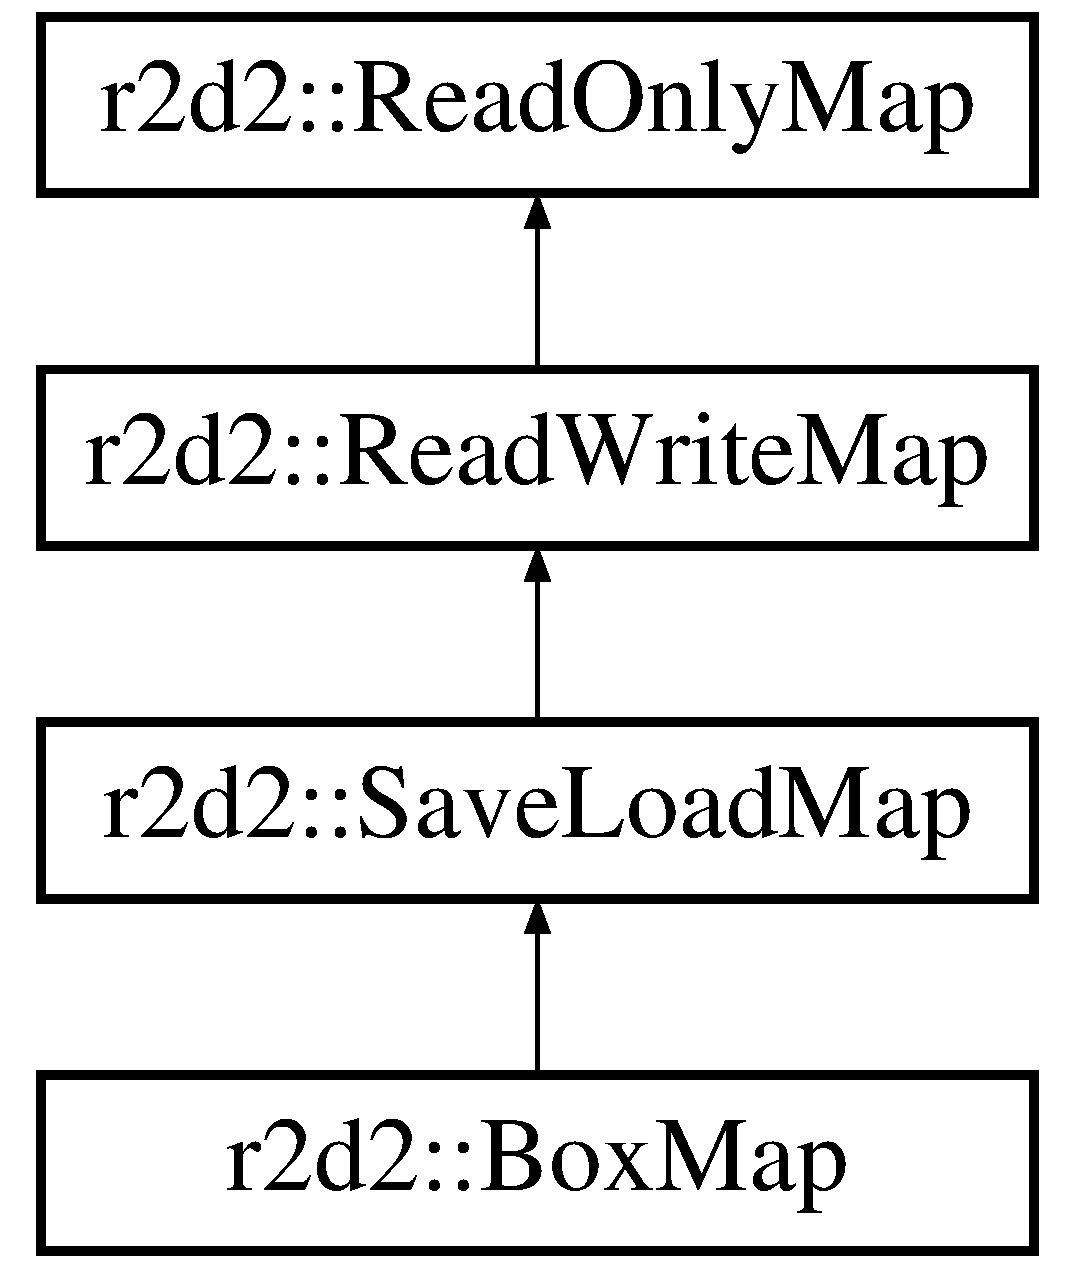
\includegraphics[height=4.000000cm]{classr2d2_1_1_read_only_map}
\end{center}
\end{figure}
\subsection*{Public Member Functions}
\begin{DoxyCompactItemize}
\item 
virtual const \hyperlink{classr2d2_1_1_box_info}{Box\+Info} \hyperlink{classr2d2_1_1_read_only_map_ae088c8f8cea0870bf3db8bbf3a0821b8}{get\+\_\+box\+\_\+info} (const Box box)=0
\begin{DoxyCompactList}\small\item\em Get Box information about a certain area. All bools are false if no information is found, overwritten with true if true is found in the map. \end{DoxyCompactList}\item 
virtual const Box \hyperlink{classr2d2_1_1_read_only_map_a322efcf80b3f461769e69cbb60a87b72}{get\+\_\+map\+\_\+bounding\+\_\+box} ()=0
\begin{DoxyCompactList}\small\item\em Scans all boxes in the map and makes a box precisely around all other boxes. \end{DoxyCompactList}\end{DoxyCompactItemize}


\subsection{Member Function Documentation}
\hypertarget{classr2d2_1_1_read_only_map_ae088c8f8cea0870bf3db8bbf3a0821b8}{}\index{r2d2\+::\+Read\+Only\+Map@{r2d2\+::\+Read\+Only\+Map}!get\+\_\+box\+\_\+info@{get\+\_\+box\+\_\+info}}
\index{get\+\_\+box\+\_\+info@{get\+\_\+box\+\_\+info}!r2d2\+::\+Read\+Only\+Map@{r2d2\+::\+Read\+Only\+Map}}
\subsubsection[{get\+\_\+box\+\_\+info(const Box box)=0}]{\setlength{\rightskip}{0pt plus 5cm}virtual const {\bf Box\+Info} r2d2\+::\+Read\+Only\+Map\+::get\+\_\+box\+\_\+info (
\begin{DoxyParamCaption}
\item[{const Box}]{box}
\end{DoxyParamCaption}
)\hspace{0.3cm}{\ttfamily [pure virtual]}}\label{classr2d2_1_1_read_only_map_ae088c8f8cea0870bf3db8bbf3a0821b8}


Get Box information about a certain area. All bools are false if no information is found, overwritten with true if true is found in the map. 

Get Box Information.


\begin{DoxyParams}{Parameters}
{\em box} & The area that is to be checked. \\
\hline
\end{DoxyParams}
\begin{DoxyReturn}{Returns}
\hyperlink{classr2d2_1_1_box_info}{Box\+Info}, the found information about the area. 
\end{DoxyReturn}


Implemented in \hyperlink{classr2d2_1_1_box_map_aa6fd512737ad45da9bc46a516807f71e}{r2d2\+::\+Box\+Map}.

\hypertarget{classr2d2_1_1_read_only_map_a322efcf80b3f461769e69cbb60a87b72}{}\index{r2d2\+::\+Read\+Only\+Map@{r2d2\+::\+Read\+Only\+Map}!get\+\_\+map\+\_\+bounding\+\_\+box@{get\+\_\+map\+\_\+bounding\+\_\+box}}
\index{get\+\_\+map\+\_\+bounding\+\_\+box@{get\+\_\+map\+\_\+bounding\+\_\+box}!r2d2\+::\+Read\+Only\+Map@{r2d2\+::\+Read\+Only\+Map}}
\subsubsection[{get\+\_\+map\+\_\+bounding\+\_\+box()=0}]{\setlength{\rightskip}{0pt plus 5cm}virtual const Box r2d2\+::\+Read\+Only\+Map\+::get\+\_\+map\+\_\+bounding\+\_\+box (
\begin{DoxyParamCaption}
{}
\end{DoxyParamCaption}
)\hspace{0.3cm}{\ttfamily [pure virtual]}}\label{classr2d2_1_1_read_only_map_a322efcf80b3f461769e69cbb60a87b72}


Scans all boxes in the map and makes a box precisely around all other boxes. 

Get the Box containing all boxes in the current map.

\begin{DoxyReturn}{Returns}
const Box, the box containing all other boxes. 
\end{DoxyReturn}


Implemented in \hyperlink{classr2d2_1_1_box_map_ac1aea64a58cdb6916ecbcb0d2ea780c2}{r2d2\+::\+Box\+Map}.



The documentation for this class was generated from the following file\+:\begin{DoxyCompactItemize}
\item 
source/include/Map\+Interface.\+hpp\end{DoxyCompactItemize}

\hypertarget{classr2d2_1_1_read_write_map}{}\section{r2d2\+:\+:Read\+Write\+Map Class Reference}
\label{classr2d2_1_1_read_write_map}\index{r2d2\+::\+Read\+Write\+Map@{r2d2\+::\+Read\+Write\+Map}}
Inheritance diagram for r2d2\+:\+:Read\+Write\+Map\+:\begin{figure}[H]
\begin{center}
\leavevmode
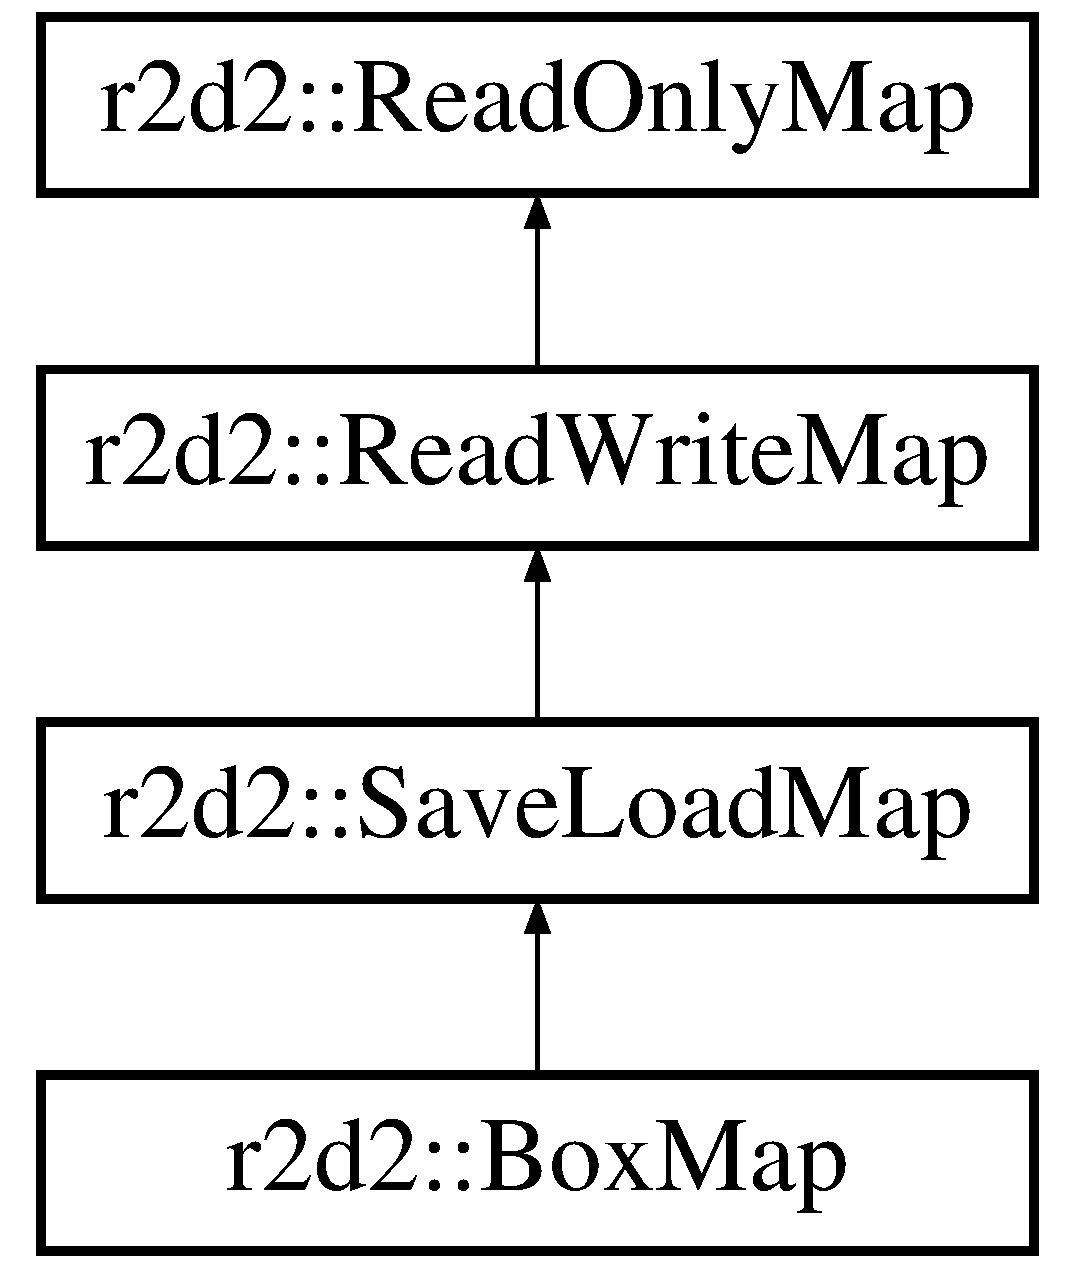
\includegraphics[height=4.000000cm]{classr2d2_1_1_read_write_map}
\end{center}
\end{figure}
\subsection*{Public Member Functions}
\begin{DoxyCompactItemize}
\item 
virtual void \hyperlink{classr2d2_1_1_read_write_map_a8169c7a36a66b824403a4df7a91d232d}{set\+\_\+box\+\_\+info} (const Box box, const \hyperlink{classr2d2_1_1_box_info}{Box\+Info} box\+\_\+info)=0
\begin{DoxyCompactList}\small\item\em Places a new box in the map with \hyperlink{classr2d2_1_1_box_info}{Box\+Info}. \end{DoxyCompactList}\end{DoxyCompactItemize}


\subsection{Member Function Documentation}
\hypertarget{classr2d2_1_1_read_write_map_a8169c7a36a66b824403a4df7a91d232d}{}\index{r2d2\+::\+Read\+Write\+Map@{r2d2\+::\+Read\+Write\+Map}!set\+\_\+box\+\_\+info@{set\+\_\+box\+\_\+info}}
\index{set\+\_\+box\+\_\+info@{set\+\_\+box\+\_\+info}!r2d2\+::\+Read\+Write\+Map@{r2d2\+::\+Read\+Write\+Map}}
\subsubsection[{set\+\_\+box\+\_\+info(const Box box, const Box\+Info box\+\_\+info)=0}]{\setlength{\rightskip}{0pt plus 5cm}virtual void r2d2\+::\+Read\+Write\+Map\+::set\+\_\+box\+\_\+info (
\begin{DoxyParamCaption}
\item[{const Box}]{box, }
\item[{const {\bf Box\+Info}}]{box\+\_\+info}
\end{DoxyParamCaption}
)\hspace{0.3cm}{\ttfamily [pure virtual]}}\label{classr2d2_1_1_read_write_map_a8169c7a36a66b824403a4df7a91d232d}


Places a new box in the map with \hyperlink{classr2d2_1_1_box_info}{Box\+Info}. 

Place new Box with \hyperlink{classr2d2_1_1_box_info}{Box\+Info} in map.


\begin{DoxyParams}{Parameters}
{\em box} & the new Box to be added. \\
\hline
{\em box\+\_\+info} & the new \hyperlink{classr2d2_1_1_box_info}{Box\+Info} thats found in that Box. \\
\hline
\end{DoxyParams}


Implemented in \hyperlink{classr2d2_1_1_box_map_ac421b31be9f2e2248127f21f3299883d}{r2d2\+::\+Box\+Map}.



The documentation for this class was generated from the following file\+:\begin{DoxyCompactItemize}
\item 
source/include/Map\+Interface.\+hpp\end{DoxyCompactItemize}

\hypertarget{classr2d2_1_1_save_load_map}{}\section{r2d2\+:\+:Save\+Load\+Map Class Reference}
\label{classr2d2_1_1_save_load_map}\index{r2d2\+::\+Save\+Load\+Map@{r2d2\+::\+Save\+Load\+Map}}
Inheritance diagram for r2d2\+:\+:Save\+Load\+Map\+:\begin{figure}[H]
\begin{center}
\leavevmode
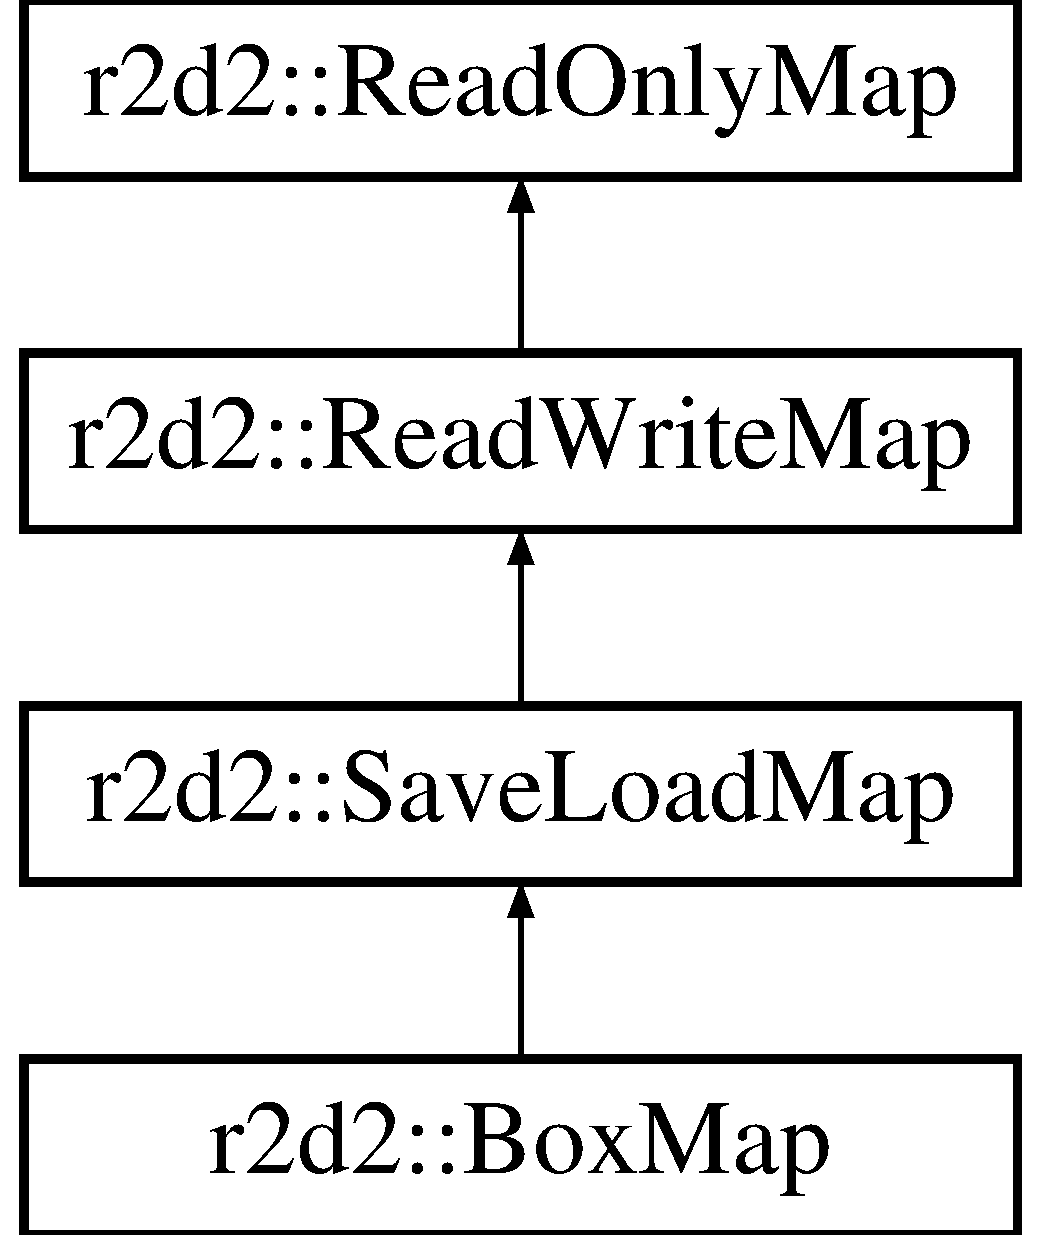
\includegraphics[height=4.000000cm]{classr2d2_1_1_save_load_map}
\end{center}
\end{figure}
\subsection*{Public Member Functions}
\begin{DoxyCompactItemize}
\item 
\hypertarget{classr2d2_1_1_save_load_map_a6739a265b27535e96d50b9889308ec2a}{}virtual void {\bfseries save} (std\+::string filename)=0\label{classr2d2_1_1_save_load_map_a6739a265b27535e96d50b9889308ec2a}

\item 
\hypertarget{classr2d2_1_1_save_load_map_ae7e67d4a8dca19cd3f96139f5b401a0a}{}virtual void {\bfseries load} (std\+::string filename)=0\label{classr2d2_1_1_save_load_map_ae7e67d4a8dca19cd3f96139f5b401a0a}

\end{DoxyCompactItemize}


The documentation for this class was generated from the following file\+:\begin{DoxyCompactItemize}
\item 
source/include/Map\+Interface.\+hpp\end{DoxyCompactItemize}

%--- End generated contents ---

% Index
\backmatter
\newpage
\phantomsection
\clearemptydoublepage
\addcontentsline{toc}{chapter}{Index}
\printindex

\end{document}
